\documentclass[10pt]{article}

\usepackage{graphicx}
\usepackage{epstopdf}
\usepackage{float}
\usepackage[T1]{fontenc}
\usepackage[titletoc]{appendix}
\usepackage[margin=0.7in]{geometry}
\usepackage{blindtext}
\usepackage[english]{babel}
\usepackage{multirow}
\usepackage{courier}
\usepackage{fancyhdr}
\usepackage{makecell}
\usepackage{caption}
\usepackage{rotating}
\usepackage{pdflscape}
\pagestyle{fancy}
\lhead{Tim Yao - ty252}

\renewcommand{\thesubsection}{\thesection.\alph{subsection}}

\usepackage{listings}
\usepackage{color}

\definecolor{dkgreen}{rgb}{0,0.6,0}
\definecolor{gray}{rgb}{0.5,0.5,0.5}
\definecolor{mauve}{rgb}{0.58,0,0.82}

\lstset{frame=tb,
  language=Verilog,
  aboveskip=3mm,
  belowskip=3mm,
  showstringspaces=false,
  columns=flexible,
  keepspaces=true,
  numbers=left,
  basicstyle={\small\ttfamily},
  keywordstyle=\color{blue},
  commentstyle=\color{dkgreen},
  stringstyle=\color{mauve},
  breaklines=false,
  breakatwhitespace=true,
  tabsize=2
}

% For monospace stuff

\title{ECE 4750 PSET 4}
\author{Tim Yao (ty252)}
\date{Nov 25, 2015}

\begin{document}
\maketitle
\newcommand*{\tableindent}{\hspace*{0.3cm}}%
Worked with Gautam Ramaswamy, Gaurab Bhattacharya, and Sacheth Hegde.
\section{Tree Network Topologies} 

\subsection{Baseline I3L Microarchitecture}
\begin{figure}[H]
\centering
{\setlength{\tabcolsep}{2pt}
\begin{tabular}{|l|c|c!{\vrule width 1.5pt}c|c|c|c|c|c|c|c|c|c|c|c|c|c|c|c|c|c|c|c|c|c|c|c|c|c|c!{\vrule width 1.5pt}}
\hline
Cycle:            & 0 & 1 & 2 & 3 & 4 & 5 & 6 & 7 & 8 & 9 & 10 & 11 & 12 & 13 & 14 & 15 & 16 & 17 & 18 & 19 & 20 & 21 & 22 & 23 & 24 & 25 & 26 & 27 & 28 \\ \hline
mul r1, r2, r3    & F & D & I & Y0& Y1& Y2& Y3& W &   &   &    &    &    &    &    &    &    &    &    &    &    &    &    &    &    &    &    &    &    \\ \hline
mul r4, r1, r5    &   & F & D & I & I & I & I & Y0& Y1& Y2& Y3 & W  &    &    &    &    &    &    &    &    &    &    &    &    &    &    &    &    &    \\ \hline
div r6, r7, r8    &   &   & F & D & D & D & D & I & Z & Z & Z  & Z  & W  &    &    &    &    &    &    &    &    &    &    &    &    &    &    &    &    \\ \hline
div r9, r10, r11  &   &   &   & F & F & F & F & D & I & I & I  & I  & Z  & Z  & Z  & Z  & W  &    &    &    &    &    &    &    &    &    &    &    &    \\ \hline
div r12, r13, r14 &   &   &   &   &   &   &   & F & D & D & D  & D  & I  & I  & I  & I  & Z  & Z  & Z  & Z  & W  &    &    &    &    &    &    &    &    \\ \hline
mul r15, r12, r16 &   &   &   &   &   &   &   &   & F & F & F  & F  & D  & D  & D  & D  & I  & I  & I  & I  & Y0 & Y1 & Y2 & Y3 & W  &    &    &    &    \\ \hline
mul r17, r15, r18 &   &   &   &   &   &   &   &   &   &   &    &    & F  & F  & F  & F  & D  & D  & D  & D  & I  & I  & I  & I  & Y0 & Y1 & Y2 & Y3 & W  \\ \hline
\end{tabular}
}
\caption{Pipeline Diagram for Baseline I3L Architecture}
\end{figure}

The total issue to commit cycle count is 27.

\subsection{Schedule Oldest Ready Instruction First on IO2L Microarchitecture}

\begin{figure}[H]
\centering
{\setlength{\tabcolsep}{2pt}
\begin{tabular}{|l!{\vrule width 1.5pt}c|c|c|c|c|c|c|c|c|c|c|c|c|c|c|c|c|c|c|c|c|c|c|c!{\vrule width 1.5pt}}
\hline
Cycle:            & 0 & 1 & 2 & 3 & 4 & 5 & 6 & 7 & 8 & 9 & 10 & 11 & 12 & 13 & 14 & 15 & 16 & 17 & 18 & 19 & 20 & 21 & 22 & 23 \\ \hline
mul r1, r2, r3    & I & Y0& Y1& Y2& Y3& W & C &   &   &   &    &    &    &    &    &    &    &    &    &    &    &    &    &    \\ \hline
mul r4, r1, r5    &   &   &   &   & I & Y0& Y1& Y2& Y3& W & C  &    &    &    &    &    &    &    &    &    &    &    &    &    \\ \hline
div r6, r7, r8    &   & I & Z & Z & Z & Z & W & r & r & r & r  & C  &    &    &    &    &    &    &    &    &    &    &    &    \\ \hline
div r9, r10, r11  &   &   &   &   &   & I & Z & Z & Z & Z & W  & r  & C  &    &    &    &    &    &    &    &    &    &    &    \\ \hline
div r12, r13, r14 &   &   &   &   &   &   &   &   &   & I & Z  & Z  & Z  & Z  & W  & C  &    &    &    &    &    &    &    &    \\ \hline
mul r15, r12, r16 &   &   &   &   &   &   &   &   &   &   &    &    &    & I  & Y0 & Y1 & Y2 & Y3 & W  & C  &    &    &    &    \\ \hline
mul r17, r15, r18 &   &   &   &   &   &   &   &   &   &   &    &    &    &    &    &    &    & I  & Y0 & Y1 & Y2 & Y3 & W  & C  \\ \hline
\end{tabular}
}
\caption{Pipeline Diagram for IO2L Architecture}
\end{figure}

The total issue to commit cycle count is 24.

\subsection{Optimal Scheduling on IO2L Microarchitecture}

\begin{figure}[H]
\centering
{\setlength{\tabcolsep}{2pt}
\begin{tabular}{|l!{\vrule width 1.5pt}c|c|c|c|c|c|c|c|c|c|c|c|c|c|c|c|c|c!{\vrule width 1.5pt}}
\hline
Cycle:            & 0 & 1 & 2 & 3 & 4 & 5 & 6 & 7 & 8 & 9 & 10 & 11 & 12 & 13 & 14 & 15 & 16 & 17 \\ \hline
mul r1, r2, r3    &   & I & Y0& Y1& Y2& Y3& W & C &   &   &    &    &    &    &    &    &    &    \\ \hline
mul r4, r1, r5    &   &   &   &   &   & I & Y0& Y1& Y2& Y3& W  & C  &    &    &    &    &    &    \\ \hline
div r6, r7, r8    &   &   &   &   & I & Z & Z & Z & Z & W & r  & r  & C  &    &    &    &    &    \\ \hline
div r9, r10, r11  &   &   &   &   &   &   &   &   & I & Z & Z  & Z  & Z  & W  & C  &    &    &    \\ \hline
div r12, r13, r14 & I & Z & Z & Z & Z & W & r & r & r & r & r  & r  & r  & r  & r  & C  &    &    \\ \hline
mul r15, r12, r16 &   &   &   &   &   &   & I & Y0& Y1& Y2& Y3 & W  & r  & r  & r  & r  & C  &    \\ \hline
mul r17, r15, r18 &   &   &   &   &   &   &   &   &   &   & I  & Y0 & Y1 & Y2 & Y3 & W  & r  & C  \\ \hline
\end{tabular}
}
\caption{Pipeline Diagram for IO2L Architecture with Optimized Scheduling}
\end{figure}

The total issue to commit cycle count is 18.

\subsection{Scheduling Comparison}

TODO!

\cleardoublepage
\section{Register Renaming}

\subsection{Architectural RAW, WAW, and WAR Dependencies}

\begin{lstlisting}
mul  r1, r2, r3
mul  r4, r1, r5
addu r6, r7, r8
mul  r1, r2, r5
addu r6, r6, r9
\end{lstlisting}

\subsection{Pipeline Diagram with Register Renaming}

\begin{figure}[H]
\centering
{\setlength{\tabcolsep}{2pt}
\begin{tabular}{|l|c|c|c|c|c|c|c|c|c|c|c|c|c|c|c|c|}
\hline
Cycle:            & 0 & 1 & 2 & 3 & 4 & 5 & 6 & 7 & 8 & 9 & 10 & 11 & 12 & 13 & 14 & 15 \\ \hline
mul  r1, r2, r3   & F & D & I & Y0& Y1& Y2& Y3& W & C &   &    &    &    &    &    &    \\ \hline
mul  r4, r1, r5   &   & F & D & i & i & i & I & Y0& Y1& Y2& Y3 & W  & C  &    &    &    \\ \hline
addu r6, r7, r8   &   &   & F & D & I & X & W & r & r & r & r  & r  & r  & C  &    &    \\ \hline
mul  r1, r2, r5   &   &   &   & F & D & I & Y0& Y1& Y2& Y3& W  & r  & r  & r  & C  &    \\ \hline
addu r6, r6, r9   &   &   &   &   & F & D & i & I & X & W & r  & r  & r  & r  & r  & C  \\ \hline
\end{tabular}
}
\caption{Pipeline Diagram with Register Renaming}
\end{figure}

\subsection{Register Renaming with Pointers in the IQ/ROB}

\begin{figure}[H]
\centering
{\setlength{\tabcolsep}{2pt}
\begin{tabular}{@{\extracolsep{3pt}}cccccccccccccclc@{}}
\hline
& \multicolumn{4}{c}{\textbf{Stage}} & \multicolumn{9}{c}{\textbf{RT}} & & \\
\cline{2-5}
\cline{6-14}
\textbf{Cycle} & \textbf{D} & \textbf{I} & \textbf{W} & \textbf{C} & \textbf{r1} & \textbf{r2} & \textbf{r3} & \textbf{r4} & \textbf{r5} & \textbf{r6} & \textbf{r7} & \textbf{r8} & \textbf{r9} & \textbf{Free List} & \textbf{IQ} \\ \hline
0 &   &   &   &   & p0 & p1 & p2 & p3 & p4 & p5 & p6 & p7 & p8 & p9,pA,pB,pC,pD &          \\ \hline
1 & 1 &   &   &   & :  & :  & :  & :  & :  & :  & :  & :  & :  & p9,pA,pB,pC,pD &          \\ \hline
2 & 2 & 1 &   &   & p9*& :  & :  & :  & :  & :  & :  & :  & :  & pA,pB,pC,pD    & p9/p1/p2 \\ \hline
3 & 3 &   &   &   & :  & :  & :  & pA*& :  & :  & :  & :  & :  & pB,pC,pD       & pA/p9*/p4\\ \hline
4 & 4 & 3 &   &   & :  & :  & :  & :  & :  & pB*& :  & :  & :  & pC,pD          & pB/p6/p7 \\ \hline
5 & 5 & 4 &   &   & pC*& :  & :  & :  & :  & :  & :  & :  & :  & pD             & pC/p1/p4 \\ \hline
6 &   & 2 & 3 &   & :  & :  & :  & :  & :  & pD*& :  & :  & :  &                & pD/pB*/p8\\ \hline
7 &   & 5 & 1 &   & :  & :  & :  & :  & :  & :  & :  & :  & :  &                &          \\ \hline
8 &   &   &   & 1 & :  & :  & :  & :  & :  & :  & :  & :  & :  &                &          \\ \hline
9 &   &   & 5 &   & :  & :  & :  & :  & :  & :  & :  & :  & :  & p0             &          \\ \hline
10&   &   & 4 &   & :  & :  & :  & :  & :  & pD & :  & :  & :  & p0             &          \\ \hline
11&   &   & 2 &   & pC & :  & :  & :  & :  & :  & :  & :  & :  & p0             &          \\ \hline
12&   &   &   & 2 & :  & :  & :  & pA & :  & :  & :  & :  & :  & p0             &          \\ \hline
13&   &   &   & 3 & :  & :  & :  & :  & :  & :  & :  & :  & :  & p0,p3          &          \\ \hline
14&   &   &   & 4 & :  & :  & :  & :  & :  & :  & :  & :  & :  & p0,p3,p5       &          \\ \hline
15&   &   &   & 5 & :  & :  & :  & :  & :  & :  & :  & :  & :  & p0,p3,p5,p9    &          \\ \hline
16&   &   &   &   & :  & :  & :  & :  & :  & :  & :  & :  & :  & p0,p3,p5,p9,pB &          \\ \hline
\end{tabular}
}
\caption{Microarchitectural State (RT/FL/IQ) for Reg Renaming with Pointers in the IQ/ROB}
\end{figure} 

\begin{figure}[H]
\centering
{\setlength{\tabcolsep}{2pt}
\begin{tabular}{@{\extracolsep{3pt}}cccccc@{}}
\hline
& \multicolumn{5}{c}{\textbf{ROB}} \\
\cline{2-6}
\textbf{Cycle} & \textbf{0} & \textbf{1} & \textbf{2} & \textbf{3} & \textbf{4} \\ \hline
0 &            &            &            &            &            \\ \hline
1 &            &            &            &            &            \\ \hline
2 & p9*/r1/p0  &            &            &            &            \\ \hline
3 &     |      & pA*/r4/p3  &            &            &            \\ \hline
4 &     |      &     |      & pB*/r6/p5  &            &            \\ \hline
5 &     |      &     |      &     |      & pC*/r1/p9* &            \\ \hline
6 &     |      &     |      &     |      &     |      & pD*/r6/pB* \\ \hline
7 &     |      &     |      & pB/r6/p5   &     |      & pD*/r6/pB  \\ \hline
8 & p9/r1/p0   &     |      &     |      & pC*/r1/p9  &     |      \\ \hline
9 &            &     |      &     |      &     |      &     |      \\ \hline
10&            &     |      &     |      &     |      & pD/r6/pB   \\ \hline
11&            &     |      &     |      & pC/r1/p9   &     |      \\ \hline
12&            & pA/r4/p3   &     |      &     |      &     |      \\ \hline
13&            &            &\textbullet &     |      &     |      \\ \hline
14&            &            &            &\textbullet &     |      \\ \hline
15&            &            &            &            &\textbullet \\ \hline
\end{tabular}
}
\caption{Microarchitectural State (ROB) for Reg Renaming with Pointers in the IQ/ROB}
\end{figure} 

\subsection{Register Renaming with Values in the IQ/ROB}

\begin{figure}[H]
\centering
{\setlength{\tabcolsep}{2pt}
\begin{tabular}{@{\extracolsep{3pt}}cccccccccccccccccccc@{}}
\hline
& \multicolumn{4}{c}{\textbf{Stage}} & \multicolumn{9}{c}{\textbf{RT}} & & \multicolumn{5}{c}{\textbf{ROB}}\\
\cline{2-5}
\cline{6-14}
\cline{16-20}
\textbf{Cycle} & \textbf{D} & \textbf{I} & \textbf{W} & \textbf{C} & \textbf{r1} & \textbf{r2} & \textbf{r3} & \textbf{r4} & \textbf{r5} & \textbf{r6} & \textbf{r7} & \textbf{r8} & \textbf{r9} & \textbf{IQ} & \textbf{0} & \textbf{1} & \textbf{2} & \textbf{3} & \textbf{4} \\ \hline
0 &   &   &   &   &    &    &    &    &    &    &    &    &    &           &        &        &        &        &        \\ \hline
1 & 1 &   &   &   &    &    &    &    &    &    &    &    &    &           &        &        &        &        &        \\ \hline
2 & 2 & 1 &   &   & p0*&    &    &    &    &    &    &    &    & p0/r2/r3  & p0*/r1 &        &        &        &        \\ \hline
3 & 3 &   &   &   &  | &    &    & p1*&    &    &    &    &    & p1/p0*/r5 &   |    & p1*/r4 &        &        &        \\ \hline
4 & 4 & 3 &   &   &  | &    &    &  | &    & p2*&    &    &    & p2/r7/r8  &   |    &   |    & p2*/r6 &        &        \\ \hline
5 & 5 & 4 &   &   & p3*&    &    &  | &    &  | &    &    &    & p3/r2/r5  &   |    &   |    &   |    & p3*/r1 &        \\ \hline
6 &   & 2 & 3 &   &  | &    &    &  | &    & p4*&    &    &    & p4/p2*/r9 &   |    &   |    &   |    &   |    & p4*/r6 \\ \hline
7 &   & 5 & 1 &   &  | &    &    &  | &    &  | &    &    &    &           &   |    &   |    & p2/r6  &   |    &   |    \\ \hline
8 &   &   &   & 1 &  | &    &    &  | &    &  | &    &    &    &           & p0/r1  &   |    &   |    &   |    &   |    \\ \hline
9 &   &   & 5 &   &  | &    &    &  | &    &  | &    &    &    &           &        &   |    &   |    &   |    &   |    \\ \hline
10&   &   & 4 &   &  | &    &    &  | &    & p4 &    &    &    &           &        &   |    &   |    &   |    & p4/r6  \\ \hline
11&   &   & 2 &   & p3 &    &    &  | &    &  | &    &    &    &           &        &   |    &   |    & p3/r1  &   |    \\ \hline
12&   &   &   & 2 &  | &    &   &$\cdot$&  &  | &    &    &    &           &        & p1/r4  &   |    &   |    &   |    \\ \hline
13&   &   &   & 3 &  | &    &    &    &    &  | &    &    &    &           &        &        &   |    &   |    &   |    \\ \hline
14&   &   &   & 4&$\cdot$&  &    &    &    &  | &    &    &    &           &        &      &\textbullet&  |    &   |    \\ \hline
15&   &   &   & 5 &    &    &    &    &    &  | &    &    &    &           &        &        &      &\textbullet&  |    \\ \hline
16&   &   &   &   &    &    &    &    &   &$\cdot$&  &    &    &           &        &        &        &    &\textbullet \\ \hline
\end{tabular}
}
\caption{Microarchitectural State for Reg Renaming with Values in the IQ/ROB}
\end{figure} 

\cleardoublepage
\section{In-Order vs. Out-of-Order Superscalar Processors}

\subsection{Performance of In-Order Dual-Issue Processor}

\begin{figure}[H]
\centering
{\setlength{\tabcolsep}{2pt}
\begin{tabular}{|l|c|c|c|c|c!{\vrule width 1.5pt}c|c|c|c|c|c|c|c|c!{\vrule width 1.5pt}}
\hline
Cycle:            & 0  & 1  & 2  & 3  & 4  & 5  & 6  & 7  & 8  & 9  & 10 & 11 & 12 & 13 \\ \hline
lw r1 , 0(r2)     & F  & D  & I  & L0 & L1 & W  & C  &    &    &    &    &    &    &    \\ \hline
mul r3, r1, r4    & F  & D  & I  & I  & I  & Y0 & Y1 & Y2 & Y3 & W  & C  &    &    &    \\ \hline
sw r3, 0(r5)      &    & F  & D  & D  & D  & D  & D  & D  & I  & S  & W  & C  &    &    \\ \hline
addiu r2, r2, 4   &    & F  & D  & D  & D  & D  & D  & D  & I  & A  & W  & C  &    &    \\ \hline
addiu r5, r5, 4   &    &    & F  & F  & F  & F  & F  & F  & D  & I  & A  & W  & C  &    \\ \hline
addiu r6, r6, -1  &    &    & F  & F  & F  & F  & F  & F  & D  & I  & B  & W  & C  &    \\ \hline
bne r6, r0, loop  &    &    &    &    &    &    &    &    & F  & D  & I  & A  & W  & C  \\ \hline
opA               &    &    &    &    &    &    &    &    & F  & *  & *  & *  & *  & *  \\ \hline
\end{tabular}
}
\caption{Pipeline Diagram for In-Order Dual-Issue Processor}
\end{figure}
As shown by the bold vertical lines, during steady state, each loop takes 9 cycles to execute. The W stage of the lw instruction is included because during looping, the W stages causes an extra cycle of "delay" between the last commit of the previous iteration and the first commit of the current iteration.

Therefore, the total number of cycles it takes to execute 64 iterations is 9*64 = 576 cycles.

\subsection{Performance of Out-of-Order Dual-Issue Processor}

\begin{figure}[H]
\centering
{\setlength{\tabcolsep}{2pt}
\begin{tabular}{|l|c|c|c|c|c!{\vrule width 1.5pt}c|c|c|c|c|c|c|c|c!{\vrule width 1.5pt}}
\hline
Cycle:            & 0  & 1  & 2  & 3  & 4  & 5  & 6  & 7  & 8  & 9  & 10 & 11 & 12 & 13 \\ \hline
lw r1 , 0(r2)     & F  & D  & I  & L0 & L1 & W  & C  &    &    &    &    &    &    &    \\ \hline
mul r3, r1, r4    & F  & D  & I  & I  & I  & Y0 & Y1 & Y2 & Y3 & W  & C  &    &    &    \\ \hline
sw r3, 0(r5)      &    & F  & D  & D  & D  & D  & D  & D  & I  & S  & W  & C  &    &    \\ \hline
addiu r2, r2, 4   &    & F  & D  & D  & D  & D  & D  & D  & I  & A  & W  & C  &    &    \\ \hline
addiu r5, r5, 4   &    &    & F  & F  & F  & F  & F  & F  & D  & I  & A  & W  & C  &    \\ \hline
addiu r6, r6, -1  &    &    & F  & F  & F  & F  & F  & F  & D  & I  & B  & W  & C  &    \\ \hline
bne r6, r0, loop  &    &    &    &    &    &    &    &    & F  & D  & I  & A  & W  & C  \\ \hline
opA               &    &    &    &    &    &    &    &    & F  & *  & *  & *  & *  & *  \\ \hline
\end{tabular}
}
\caption{Pipeline Diagram for Out-of-Order Dual-Issue Processor}
\end{figure}
As shown by the bold vertical lines, during steady state, each loop takes 9 cycles to execute. The W stage of the lw instruction is included because during looping, the W stages causes an extra cycle of "delay" between the last commit of the previous iteration and the first commit of the current iteration.

Therefore, the total number of cycles it takes to execute 64 iterations is 9*64 = 576 cycles.

\subsection{Instruction Level Parallelism}

\begin{figure}[H]
\begin{center}
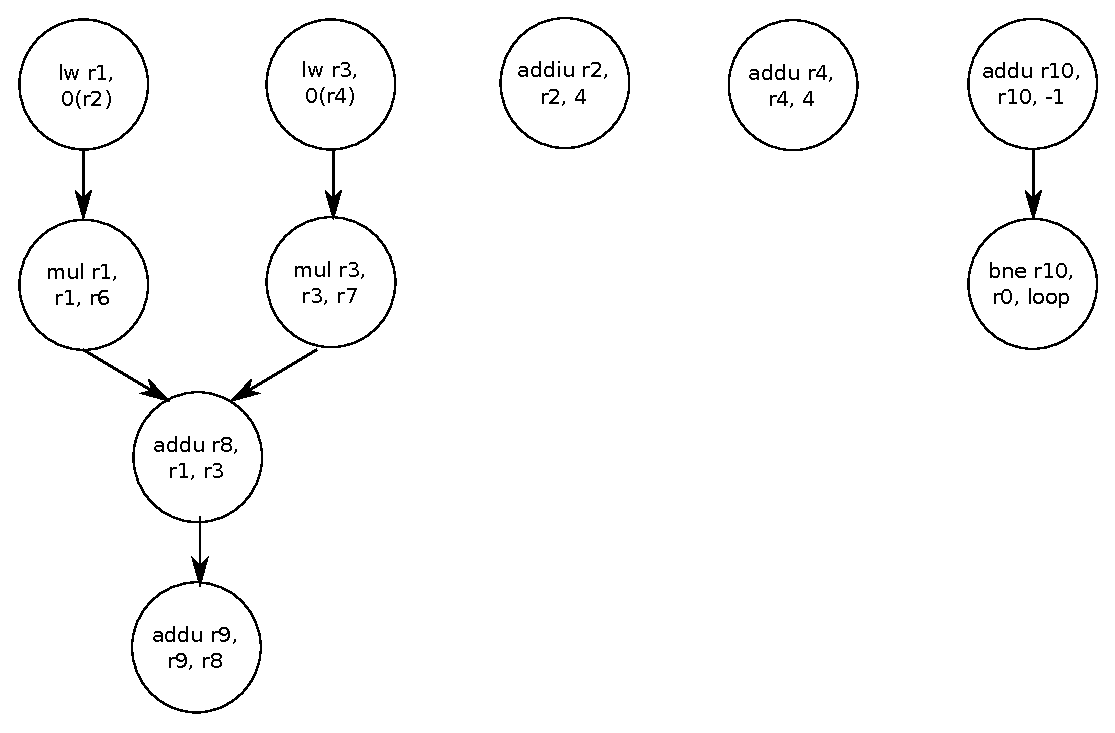
\includegraphics[scale=0.5]{singleiteri.eps}
\label{default}
\end{center}
\caption{Instruction Dependency Graph for Single Iteration}
\end{figure}

\begin{figure}[H]
\begin{center}
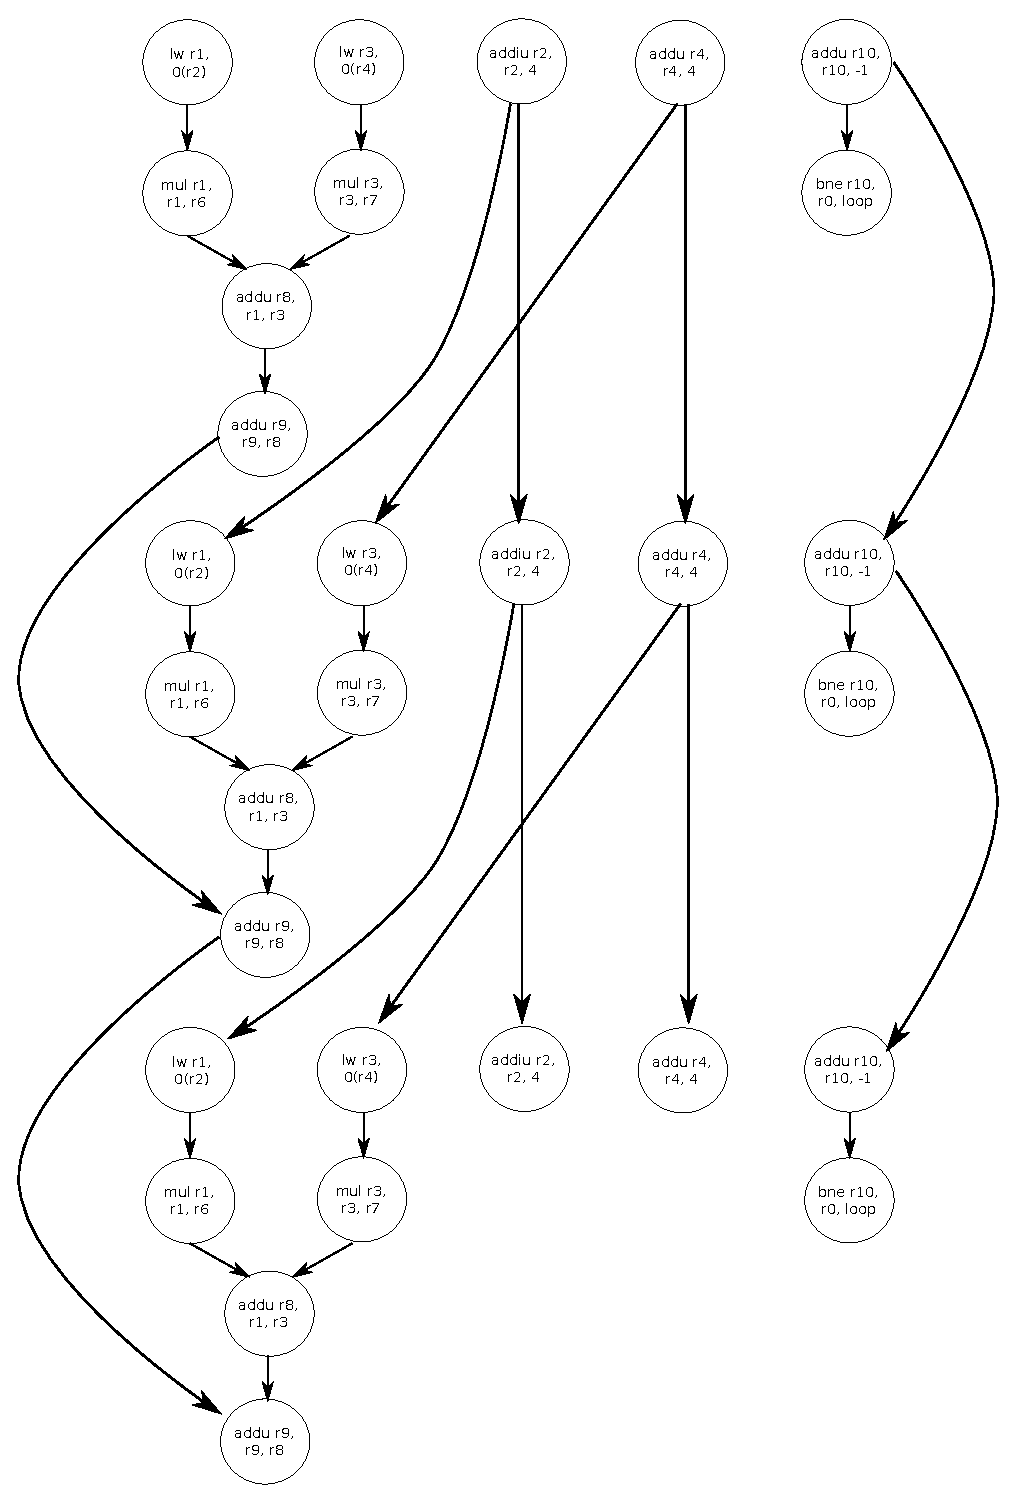
\includegraphics[scale=0.7]{threeiteri.eps}
\label{default}
\end{center}
\caption{Instruction Dependency Graph for Three Iterations}
\end{figure}

\cleardoublepage
\section{Branch Prediction}

\subsection{Two-Bit Saturating Counter Branch History Table}

\begin{figure}[H]
\centering
{
\begin{tabular}{@{\extracolsep{3pt}}cclcclcclcc@{}}
\hline
& & \multicolumn{3}{c}{\textbf{Branch B0}} & \multicolumn{3}{c}{\textbf{Branch B1}} & \multicolumn{3}{c}{\textbf{Branch B2}}\\
\cline{3-5}
\cline{6-8}
\cline{9-11}
i & src[i] & \textbf{BHT} & \textbf{P} & \textbf{A} & \textbf{BHT} & \textbf{P} & \textbf{A} & \textbf{BHT} & \textbf{P} & \textbf{A} \\ \hline
0 & 0 & WT& T & T & WT& T & T & WT& T & T \\ \hline
1 & 0 & ST& T & T & ST& T & T & ST& T & T \\ \hline
2 & 12& ST& T & NT& ST& T & NT& ST& T & T \\ \hline
3 & 15& WT& T & NT& WT& T & NT& ST& T & T \\ \hline
4 & 0 &WNT& NT& T &WNT& NT& T & ST& T & T \\ \hline
5 & 0 & WT& T & T & WT& T & T & ST& T & T \\ \hline
6 & 11& ST& T & NT& ST& T & NT& ST& T & T \\ \hline
7 & 17& WT& T & NT& WT& T & NT& ST& T & T \\ \hline
8 & 0 &WNT& NT& T &WNT& NT& T & ST& T & T \\ \hline
9 & 0 & WT& T & T & WT& T & T & ST& T & T \\ \hline
10& 11& ST& T & NT& ST& T & NT& ST& T & T \\ \hline
11& 13& WT& T & NT& WT& T & NT& ST& T & T \\ \hline
12& 9 &WNT& NT& T &WNT& NT& NT& ST& T & T \\ \hline
13& 0 & WT& T & T &SNT& NT& T & ST& T & T \\ \hline
14& 12& ST& T & NT&WNT& NT& NT& ST& T & T \\ \hline
15& 15& WT& T & NT&SNT& NT& NT& ST& T & T \\ \hline
16& 0 &WNT& NT& T &SNT& NT& T & ST& T & T \\ \hline
17& 8 & WT& T & T &WNT& NT& NT& ST& T & T \\ \hline
18& 12& ST& T & NT&SNT& NT& NT& ST& T & T \\ \hline
19& 18& WT& T & NT&SNT& NT& NT& ST& T & NT\\ \hline
\end{tabular}
}
\caption{Two-Bit Saturating Counter BHT Execution}
\end{figure}

\subsection{Two-Level Adaptive Branch Predictor to Exploit Temporal Correlation}

\begin{figure}[H]
\centering
{\setlength{\tabcolsep}{3pt}
\begin{tabular}{@{\extracolsep{3pt}}ccclccclccclcc@{}}
\hline
& & \multicolumn{4}{c}{\textbf{Branch B0}} & \multicolumn{4}{c}{\textbf{Branch B1}} & \multicolumn{4}{c}{\textbf{Branch B2}}\\
\cline{3-6}
\cline{7-10}
\cline{11-14}
i & src[i] & \textbf{BHSRT} & \textbf{BHT} & \textbf{P} & \textbf{A} & \textbf{BHSRT} & \textbf{BHT} & \textbf{P} & \textbf{A} & \textbf{BHSRT} & \textbf{BHT} & \textbf{P} & \textbf{A} \\ \hline
0 & 0 & 000 & WT& T & T & 000 & WT& T & T & 000 & WT& T & T \\ \hline
1 & 0 & 001 & WT& T & T & 001 & WT& T & T & 001 & WT& T & T \\ \hline
2 & 12& 011 & WT& T & NT& 011 & WT& T & NT& 011 & WT& T & T \\ \hline
3 & 15& 110 & WT& T & NT& 110 & WT& T & NT& 111 & WT& T & T \\ \hline
4 & 0 & 100 & WT& T & T & 100 & WT& T & T & 111 & ST& T & T \\ \hline
5 & 0 & 101 & WT& T & T & 101 & WT& T & T & 111 & ST& T & T \\ \hline
6 & 11& 011 &WNT& NT& NT& 011 &WNT& NT& NT& 111 & ST& T & T \\ \hline
7 & 17& 110 &WNT& NT& NT& 110 &WNT& NT& NT& 111 & ST& T & T \\ \hline
8 & 0 & 100 & ST& T & T & 100 & ST& T & T & 111 & ST& T & T \\ \hline
9 & 0 & 101 & ST& T & T & 101 & ST& T & T & 111 & ST& T & T \\ \hline
10& 11& 011 &SNT& NT& NT& 011 &SNT& NT& NT& 111 & ST& T & T \\ \hline
11& 13& 110 &SNT& NT& NT& 110 &SNT& NT& NT& 111 & ST& T & T \\ \hline
12& 9 & 100 & ST& T & T & 100 & ST& T & NT& 111 & ST& T & T \\ \hline
13& 0 & 101 & ST& T & T & 000 & ST& T & T & 111 & ST& T & T \\ \hline
14& 12& 011 &SNT& NT& NT& 001 & ST& T & NT& 111 & ST& T & T \\ \hline
15& 15& 110 &SNT& NT& NT& 010 & WT& T & NT& 111 & ST& T & T \\ \hline
16& 0 & 100 & ST& T & T & 100 & WT& T & T & 111 & ST& T & T \\ \hline
17& 8 & 101 & ST& T & T & 001 & WT& T & NT& 111 & ST& T & T \\ \hline
18& 12& 011 &SNT& NT& NT& 010 &WNT& NT& NT& 111 & ST& T & T \\ \hline
19& 18& 110 &SNT& NT& NT& 100 & ST& T & NT& 111 & ST& T & NT\\ \hline
\end{tabular}
}
\caption{Two-Level BHT for Temporal Correlation Execution}
\end{figure}

\subsection{Two-Level Adaptive Branch Predictor to Exploit Spatial Correlation}

\begin{figure}[H]
\centering
{\setlength{\tabcolsep}{3pt}
\begin{tabular}{@{\extracolsep{3pt}}ccclccclccclcc@{}}
\hline
& & \multicolumn{4}{c}{\textbf{Branch B0}} & \multicolumn{4}{c}{\textbf{Branch B1}} & \multicolumn{4}{c}{\textbf{Branch B2}}\\
\cline{3-6}
\cline{7-10}
\cline{11-14}
i & src[i] & \textbf{BHSR} & \textbf{BHT} & \textbf{P} & \textbf{A} & \textbf{BHSR} & \textbf{BHT} & \textbf{P} & \textbf{A} & \textbf{BHSR} & \textbf{BHT} & \textbf{P} & \textbf{A} \\ \hline
0 & 0 & 0  & WT& T & T & 1  & WT& T & T & 1  & WT& T & T \\ \hline
1 & 0 & 1  & WT& T & T & 1  & ST& T & T & 1  & ST& T & T \\ \hline
2 & 12& 1  & ST& T & NT& 0  & WT& T & NT& 0  & WT& T & T \\ \hline
3 & 15& 1  & WT& T & NT& 0  &WNT& NT& NT& 0  & ST& T & T \\ \hline
4 & 0 & 1  &WNT& NT& T & 1  & ST& T & T & 1  & ST& T & T \\ \hline
5 & 0 & 1  & WT& T & T & 1  & ST& T & T & 1  & ST& T & T \\ \hline
6 & 11& 1  & ST& T & NT& 0  &SNT& NT& NT& 0  & ST& T & T \\ \hline
7 & 17& 1  & WT& T & NT& 0  &SNT& NT& NT& 0  & ST& T & T \\ \hline
8 & 0 & 1  &WNT& NT& T & 1  & ST& T & T & 1  & ST& T & T \\ \hline
9 & 0 & 1  & WT& T & T & 1  & ST& T & T & 1  & ST& T & T \\ \hline
10& 11& 1  & ST& T & NT& 0  &SNT& NT& NT& 0  & ST& T & T \\ \hline
11& 13& 1  & WT& T & NT& 0  &SNT& NT& NT& 0  & ST& T & T \\ \hline
12& 9 & 1  &WNT& NT& T & 1  & ST& T & NT& 0  & ST& T & T \\ \hline
13& 0 & 1  & WT& T & T & 1  & WT& T & T & 1  & ST& T & T \\ \hline
14& 12& 1  & ST& T & NT& 0  &SNT& NT& NT& 0  & ST& T & T \\ \hline
15& 15& 1  & WT& T & NT& 0  &SNT& NT& NT& 0  & ST& T & T \\ \hline
16& 0 & 1  &WNT& NT& T & 1  & ST& T & T & 1  & ST& T & T \\ \hline
17& 8 & 1  & WT& T & T & 1  & ST& T & NT& 0  & ST& T & T \\ \hline
18& 12& 1  & ST& T & NT& 0  &SNT& NT& NT& 0  & ST& T & T \\ \hline
19& 18& 1  & WT& T & NT& 0  &SNT& NT& NT& 0  & ST& T & NT\\ \hline
\end{tabular}
}
\caption{Two-Level BHT for Spatial Correlation Execution}
\end{figure}

\subsection{Branch Predictor Comparison}

\begin{figure}[H]
\centering
{\setlength{\tabcolsep}{3pt}
\begin{tabular}{lccc}
\hline
& \textbf{Two-Bit FSM} & \textbf{Two-Level Temporal} & \textbf{Two-Level Spatial} \\
& \textbf{Accuracy} & \textbf{Accuracy} & \textbf{Accuracy} \\ \hline
\textbf{Branch B0}    & 30\%& 90\%& 30\%\\ \hline
\textbf{Branch B1}    & 50\%& 65\%& 85\%\\ \hline
\textbf{Branch B2}    & 95\%& 95\%& 95\%\\ \hline
\textbf{All Branches} & 58\%& 83\%& 70\%\\ \hline
\end{tabular}
}
\caption{Summary of Branch Predictor Accuracies}
\end{figure}

\end{document}